% Created by: Jmol 12.0.RC26_dev  2010-07-14 15:28
% Creation date: 2010-07-17, 15:05
% File created: c:/temp/test1.idtf (1092563 bytes)


\documentclass[12pt,letter]{article}
\usepackage{hyperref}
\usepackage[3D]{movie15}
\usepackage{verbatim}
\usepackage[pdftex]{graphicx}
\pagestyle{empty}
\begin{document}
 \begin{center}

First, the U3D file... If you see nothing here, get an Adobe update. I'm using Acrobaat 9.3.3 for this.

  \includemovie[
   label=test1,
    autoplay,
    repeat=1,
    toolbar=false,
% this next one is related to the zoom
3Droo=121.74815,   
% this next is the center for the model rotation
% it's been adjusted and is not the actual xyz coordinate in the model file
3Dcoo= 0.0 0.0 0.0,
% this is the camera angle -- straight down the Z axis
3Dc2c=0.0 0.0 1.0,
% this is setting the aperature angle 
3Daac=16.260204,
% camera tilt -- not used.
% 3Droll=0.0,
% background color in rgb
3Dbg=0 0 0,
% lighitng -- no useful options here, apparently
3Dlights=Headlamp,
inline=true,
  ]{0.6\textwidth}{0.6\textwidth}{test1.u3d}
%  \\
%\movieref[3Dcalculate]{test1}{Click here!}

.

This is just a simple example. All I did was to use "write test1.idtf" and then edit the file that was created with this additional text. Also, I ran idtfConverer.exe to convert the IDTF file to U3D format for insertion here.

.

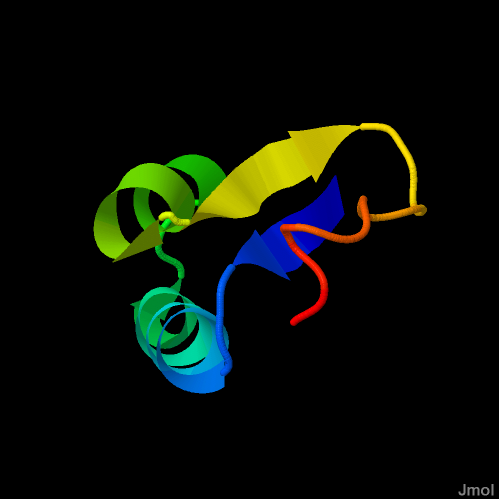
\includegraphics[scale=0.25]{test1.png}

.

That's about the extent of my knowledge of TeX.


\end{center}
\end{document}
\begin{comment}
/****** Jmol Embedded Script **** 
# Jmol state version 12.0.RC26_dev  2010-07-14 15:28;

function _setWindowState() {
# height 499;
# width 499;
  stateVersion = 1200000;
  background [x000000];
  axis1Color = "[xff0000]";
  axis2Color = "[x008000]";
  axis3Color = "[x0000ff]";
  set ambientPercent 45;
  set diffusePercent 84;
  set specular true;
  set specularPercent 22;
  set specularPower 40;
  set specularExponent 6;
  set zShadePower 1;
  statusReporting  = true;
}

function _setFileState() {

  set allowEmbeddedScripts false;
  set appendNew true;
  set appletProxy "";
  set applySymmetryToBonds false;
  set autoBond true;
  set bondRadiusMilliAngstroms 150;
  set bondTolerance 0.45;
  set defaultLattice {0.0 0.0 0.0};
  set defaultLoadFilter "";
  set defaultLoadScript "";
  set defaultVDW Auto;
  set forceAutoBond false;
  #set defaultDirectory "C:/jmol-dev/workspace/Jmol/bobtest";
  #set loadFormat "http://www.rcsb.org/pdb/files/%FILE.pdb.gz";
  #set smilesUrlFormat "http://cheminfov.informatics.indiana.edu/rest/thread/d3.py/SMILES/%FILE";
  #set edsUrlFormat "http://eds.bmc.uu.se/eds/dfs/%LC13/%LCFILE/%LCFILE.omap";
  #set edsUrlCutoff "load('http://eds.bmc.uu.se/eds/dfs/%LC13/%LCFILE/%LCFILE.sfdat').lines.find('MAP_SIGMA').split(' ')[2]";
  set minBondDistance 0.4;
  set minimizationCriterion  0.0010;
  set minimizationSteps  100;
  set pdbGetHeader false;
  set pdbSequential false;
  set percentVdwAtom 23;
  set smallMoleculeMaxAtoms 40000;
  set smartAromatic true;
  load /*file*/"./1crn.pdb";

}

function _setVariableState() {

   set defaultanglelabel "%VALUE %UNITS";
   set defaultcolorscheme "Jmol";
   set defaultdistancelabel "%VALUE %UNITS";
   set defaultdrawarrowscale 0.5;
   set defaultlattice "{0 0 0}";
   set defaultloadfilter "";
   set defaultloadscript "";
   set defaulttorsionlabel "%VALUE %UNITS";
   set defaulttranslucent 0.5;
   set defaultvdw "Auto";
  set allowembeddedscripts true;
  set allowrotateselected false;
  set appletproxy "";
  set applysymmetrytobonds false;
  set atompicking true;
  set atomtypes "";
  set autobond true;
  set autofps false;
  set axes window;
  set axesmode 0;
  set axesscale 2.0;
  set bondmodeor false;
  set bondradiusmilliangstroms 150;
  set bondtolerance 0.45;
  set cartoonbaseedges false;
  set cartoonrockets false;
  set chaincasesensitive false;
  set dataseparator "~~~";
  set delaymaximumms 0;
  set dipolescale 1.0;
  set disablepopupmenu false;
  set displaycellparameters true;
  set dotdensity 3;
  set dotscale 1;
  set dotsselectedonly false;
  set dotsurface true;
  set dragselected false;
  set drawhover false;
  set drawpicking false;
  set dynamicmeasurements false;
  set ellipsoidarcs false;
  set ellipsoidaxes false;
  set ellipsoidaxisdiameter 0.02;
  set ellipsoidball true;
  set ellipsoiddotcount 200;
  set ellipsoiddots false;
  set ellipsoidfill false;
  set forceautobond false;
  set gestureswipefactor 1.0;
  set greyscalerendering false;
  set hbondsangleminimum 90.0;
  set hbondsbackbone false;
  set hbondsdistancemaximum 3.25;
  set hbondsrasmol true;
  set hbondssolid false;
  set helixstep 1;
  set helppath "http://chemapps.stolaf.edu/jmol/docs/index.htm";
  set hermitelevel 0;
  set hidenameinpopup false;
  set hidenavigationpoint false;
  set highresolution false;
  set historylevel 0;
  set hoverdelay 0.5;
  set imagestate true;
  set iskiosk false;
  set isosurfacepropertysmoothing true;
  set justifymeasurements false;
  set loadatomdatatolerance 0.01;
  set logcommands false;
  set logfile "";
  set loggestures false;
  set measureallmodels false;
  set measurementlabels true;
  set messagestylechime false;
  set minbonddistance 0.4;
  set minimizationcriterion 0.0010;
  set minimizationrefresh true;
  set minimizationsilent false;
  set minimizationsteps 100;
  set monitorenergy false;
  set navigatesurface false;
  set navigationperiodic false;
  set navigationspeed 5.0;
  set pdbgetheader false;
  set pdbsequential false;
  set percentvdwatom 23;
  set pickingspinrate 10;
  set picklabel "";
  set pointgroupdistancetolerance 0.2;
  set pointgrouplineartolerance 8.0;
  set propertyatomnumbercolumncount 0;
  set propertyatomnumberfield 0;
  set propertycolorscheme "roygb";
  set propertydatacolumncount 0;
  set propertydatafield 0;
  set quaternionframe "p";
  set rangeselected false;
  set ribbonaspectratio 16;
  set ribbonborder false;
  set rocketbarrels false;
  set saveproteinstructurestate true;
  set selectallmodels true;
  set selecthetero true;
  set selecthydrogen true;
  set sheetsmoothing 1.0;
  set showhiddenselectionhalos false;
  set showhydrogens true;
  set showkeystrokes true;
  set showmeasurements true;
  set showmultiplebonds true;
  set shownavigationpointalways false;
  set slabbyatom false;
  set slabbymolecule false;
  set smallmoleculemaxatoms 40000;
  set smartaromatic true;
  set solventprobe false;
  set solventproberadius 1.2;
  set ssbondsbackbone false;
  set stereodegrees -5;
  set strandcountformeshribbon 7;
  set strandcountforstrands 5;
  set strutdefaultradius 0.3;
  set strutlengthmaximum 7.0;
  set strutsmultiple false;
  set strutspacing 6;
  set testflag1 false;
  set testflag2 false;
  set testflag3 false;
  set testflag4 false;
  set tracealpha true;
  set usearcball false;
  set useminimizationthread true;
  set usenumberlocalization true;
  set vectorscale 1.0;
  set vibrationscale 0.5;
  set wireframerotation false;
  set zoomlarge true;

#user-defined variables; 
# --no global user variables defined--;

# label defaults;
  select none;
  color label none;
  background label none;
  set labelOffset 4 4;
  set labelAlignment left;
  set labelPointer off;
  font label 13.0 SansSerif Plain;

}

function _setModelState() {

  select ({0:13});
  color atoms opaque [x0000ff];
  select ({146:152});
  color atoms opaque [x00ff20];
  select ({54:69});
  color atoms opaque [x00c0ff];
  select ({245:252});
  color atoms opaque [xfff000];
  select ({84:94});
  color atoms opaque [x00ffe0];
  select ({223:236});
  color atoms opaque [xf0f000];
  select ({282:292});
  color atoms opaque [xff6000];
  select ({160:173});
  color atoms opaque [x20ff00];
  select ({174:181});
  color atoms opaque [x40ff00];
  select ({153:159});
  color atoms opaque [x00ff00];
  select ({182:187});
  color atoms opaque [x60ff00];
  select ({188:199});
  color atoms opaque [x80ff00];
  select ({237:244});
  color atoms opaque [xffff00];
  select ({301:312});
  color atoms opaque [xff2000];
  select ({116:126});
  color atoms opaque [x00ff80];
  select ({95:109});
  color atoms opaque [x00ffc0];
  select ({26:38});
  color atoms opaque [x0060ff];
  select ({253:263});
  color atoms opaque [xffe000];
  select ({200:211});
  color atoms opaque [xa0ff00];
  select ({76:83});
  color atoms opaque [x00ffff];
  select ({212:218});
  color atoms opaque [xc0ff00];
  select ({219:222});
  color atoms opaque [xe0ff00];
  select ({14:19});
  color atoms opaque [x0020ff];
  select ({269:275});
  color atoms opaque [xffa000];
  select ({70:75});
  color atoms opaque [x00e0ff];
  select ({127:141});
  color atoms opaque [x00ff60];
  select ({47:53});
  color atoms opaque [x00a0ff];
  select ({110:115});
  color atoms opaque [x00ffa0];
  select ({276:281});
  color atoms opaque [xff8000];
  select ({293:300});
  color atoms opaque [xff4000];
  select ({142:145});
  color atoms opaque [x00ff40];
  select ({39:46});
  color atoms opaque [x0080ff];
  select ({313:326});
  color atoms opaque [xff0000];
  select ({20:25});
  color atoms opaque [x0040ff];
  select ({264:268});
  color atoms opaque [xffc000];
  select ({0:326});
  Spacefill 0.0;
  select BONDS ({0:336});
  wireframe 0.0;

  measures delete;
  select *; set measures nanometers;
  font measures 15.0 SansSerif Plain;

  select ({0:326});
  Cartoon on;

  boundBox off;
  font boundBox 14.0 SansSerif Plain;
  boundBox off;

  unitcell off;
  font unitcell 14.0 SansSerif Plain;
  unitcell off;

  frank on;
  font frank 16.0 SansSerif Bold;
  set fontScaling false;

}

function _setPerspectiveState() {
  set perspectiveModel 11;
  set scaleAngstromsPerInch 0.0;
  set perspectiveDepth true;
  set visualRange 5.0;
  set cameraDepth 3.0;
  boundbox corners {-3.0970001 -0.51600075 -7.4219995} {24.284 20.937 19.58} # volume = 15861.099;
  center {10.5935 10.2105 6.079};
  moveto -1.0 {0 0 1 0} 100.0 0.1 0.1 {10.5935 10.2105 6.079} 17.392593 {16.526886 12.970795 15.955903} 106.60232 -83.66469 84.060776;
  save orientation "default"
  moveto 0.0 {0 0 1 0} 100.0 0.1 0.1 {10.5935 10.2105 6.079} 17.392593 {16.526886 12.970795 15.955903} 18.488773 -8.601238 84.060776;;
  slab 100;depth 0;
  set spinX 0; set spinY 30; set spinZ 0; set spinFps 30;  set navX 0; set navY 0; set navZ 0; set navFps 10;
}

function _setSelectionState() {
  select ({0:326});
  set hideNotSelected false;
}

function _setState() {
  initialize;
  set refreshing false;
  _setWindowState;
  _setFileState;
  _setVariableState;
  _setModelState;
  _setPerspectiveState;
  _setSelectionState;
  set refreshing true;
  set antialiasDisplay false;
  set antialiasTranslucent true;
  set antialiasImages true;
}

_setState;

**/
\end{comment}